\documentclass{article}
%\usepackage[a4paper,top=3.5cm,bottom=3cm,left=3.6cm,right=3.6cm]{geometry}

\usepackage{fancyhdr}
\usepackage{extramarks}
\usepackage{amsmath}
\usepackage{amsthm}
\usepackage{amsfonts}
\usepackage{tikz}
\usetikzlibrary{arrows}
\usepackage{tikz}
\usepackage[plain]{algorithm}
\usepackage{algpseudocode}
\usepackage{enumitem}
\usepackage{amsmath}
\usepackage{caption}  
\usepackage{pgf, tikz}
\usetikzlibrary{arrows, automata}




\usetikzlibrary{automata,positioning}

\usepackage{listings}
\usepackage{xcolor}
 
\definecolor{codegreen}{rgb}{0,0.7,0}
\definecolor{codegray}{rgb}{0.5,0.5,0.5}
\definecolor{codepurple}{rgb}{0.58,0,0.82}
\definecolor{backcolour}{rgb}{0.95,0.95,0.92}

\definecolor{deepblue}{rgb}{0,0,0.5}
\definecolor{deepred}{rgb}{0.6,0,0}
\definecolor{deepgreen}{rgb}{0,0.5,0}

\makeatletter
\newcommand{\skipitems}[1]{%
  \addtocounter{\@enumctr}{#1}%
}
\makeatother 

\lstdefinestyle{mystyle}{
    backgroundcolor=\color{backcolour},   
    commentstyle=\color{codegreen},
    keywordstyle=\color{deepblue},
    numberstyle=\tiny\color{codegray},
    stringstyle=\color{deepgreen},
    basicstyle=\ttfamily\footnotesize,
    breakatwhitespace=false,         
    breaklines=true,                 
    captionpos=b,                    
    keepspaces=true,                 
    numbers=left,                    
    numbersep=5pt,                  
    showspaces=false,                
    showstringspaces=false,
    showtabs=false,                  
    tabsize=2
}
 
\lstset{style=mystyle}

\newenvironment{rcases}
  {\left.\begin{aligned}}
  {\end{aligned}\right\rbrace}
%
% Basic Document Settings
%

\topmargin=-0.45in
\evensidemargin=0in
\oddsidemargin=0in
\textwidth=6.5in
\textheight=9.0in
\headsep=0.25in

\linespread{1.1}

\pagestyle{fancy}
\lhead{\textbf{Luca Tomei} $\ $- $\ $\textbf{Andrea Aurizi}}
%\chead{\hmwkClass\ (\hmwkClassInstructor\ \hmwkClassTime): \hmwkTitle}
\chead{\hmwkClass : \hmwkTitle}
\rhead{\firstxmark}
\lfoot{\lastxmark}
\cfoot{\thepage}

\renewcommand\headrulewidth{0.4pt}
\renewcommand\footrulewidth{0.4pt}

\setlength\parindent{0pt}

%
% Create Problem Sections
%

\newcommand{\enterProblemHeader}[1]{
    \nobreak\extramarks{}{Problem \arabic{#1} continued on next page\ldots}\nobreak{}
    \nobreak\extramarks{Problem \arabic{#1} (continued)}{Problem \arabic{#1} continued on next page\ldots}\nobreak{}
}

\newcommand{\exitProblemHeader}[1]{
    \nobreak\extramarks{Problem \arabic{#1} (continued)}{Problem \arabic{#1} continued on next page\ldots}\nobreak{}
    \stepcounter{#1}
    \nobreak\extramarks{Problem \arabic{#1}}{}\nobreak{}
}

\setcounter{secnumdepth}{0}
\newcounter{partCounter}
\newcounter{homeworkProblemCounter}
\setcounter{homeworkProblemCounter}{1}
\nobreak\extramarks{Problem \arabic{homeworkProblemCounter}}{}\nobreak{}

%
% Homework Problem Environment
%
% This environment takes an optional argument. When given, it will adjust the
% problem counter. This is useful for when the problems given for your
% assignment aren't sequential. See the last 3 problems of this template for an
% example.
%
\newenvironment{homeworkProblem}[1][-1]{
    \ifnum#1>0
        \setcounter{homeworkProblemCounter}{#1}
    \fi
    \section{Problem \arabic{homeworkProblemCounter}}
    \setcounter{partCounter}{1}
    \enterProblemHeader{homeworkProblemCounter}
}{
    \exitProblemHeader{homeworkProblemCounter}
}

%
% Homework Details
%   - Title
%   - Due date
%   - Class
%   - Section/Time
%   - Instructor
%   - Author
%
\newcommand{\hmwkTitle}{Homework\ \#1}
\newcommand{\hmwkDueDate}{December 5, 2019}
\newcommand{\hmwkClass}{Algorithm Design}
\newcommand{\hmwkClassTime}{}
\newcommand{\hmwkClassInstructor}{Professor \textbf{Stefano Leonardi}}	
\newcommand{\hmwkAuthorName}{\textbf{Luca Tomei} \and \textbf{Andrea Aurizi}}

%
% Title Page
%

\title{
    \vspace{2in}
    \textmd{\textbf{\hmwkClass:\ \hmwkTitle}}\\
    \normalsize\vspace{0.1in}\small{Due\ on\ \hmwkDueDate\ at 3:10pm}\\
    \vspace{0.1in}\large{\textit{\hmwkClassInstructor\ \hmwkClassTime}}
    \vspace{3in}
}

\author{\textbf{Luca Tomei} \and \textbf{Andrea Aurizi}}
\date{}

\renewcommand{\part}[1]{\textbf{\large Part \Alph{partCounter}}\stepcounter{partCounter}\\}

%
% Various Helper Commands
%

% Useful for algorithms
\newcommand{\alg}[1]{\textsc{\bfseries \footnotesize #1}}

% For derivatives
\newcommand{\deriv}[1]{\frac{\mathrm{d}}{\mathrm{d}x} (#1)}

% For partial derivatives
\newcommand{\pderiv}[2]{\frac{\partial}{\partial #1} (#2)}

% Integral dx
\newcommand{\dx}{\mathrm{d}x}

% Alias for the Solution section header
\newcommand{\solution}{\textbf{\large Solution}}

% Probability commands: Expectation, Variance, Covariance, Bias
\newcommand{\E}{\mathrm{E}}
\newcommand{\Var}{\mathrm{Var}}
\newcommand{\Cov}{\mathrm{Cov}}
\newcommand{\Bias}{\mathrm{Bias}}

\begin{document}

\maketitle

\pagebreak

\iffalse	SPIEGAZIONE ESERCIZIO 1
Si parte dall'ultima colonna della matrice in input, perché è l'unica cassa che non dipende dalle altre, e si inizializzano a 0 i costi.
La riga corrispondente sarà i = 0,  una riga in cui i determina il corrente guadagno. In tal caso, procedendo con il gioco, il guadagno sarà comunque nullo, poiché ad esempio si puo trovare 
un price 2 ma le prime due casse costavano 1 ognuna quindi sono arrivato
ad avere guadagno 0 all'ultima cassa.
La richiesta è: dato questo gioco dove sono presenti casse con determinati costi 
e i premi che si possono trovare che vanno da 0 a n, la soluzione sta nel trovare 
l'expected optimal reward di giocare a tale gioco.

Presa una matrice 3x3:
-   partendo dall'ultima colonnna (perché è l'unica cassa che non dipende dalle 
    altre) infatti ad esempio la penultima colonna dipenderà dall'utlima cassa,
    la terzultima dalla penultima che poi dipenderà dall'ultima e così via. Questo
    perché prima di aprire la cassa corrente e quella dopo va fatta tale operaz:
    -   Parto dall'ultima cassa facendo finta che costi 0
    -   La riga corrispondente sarà i = 0 => è una riga in cui 'i' determina il mio
        corrente guadagno. In tal caso giocando ho guadagnato 0, ad esempio ho trovato
        un price 2 ma le prime due casse costavano 1 ognuna quindi sono arrivato
        ad avere guadagno 0 all'ultima cassa.
    -   Ora occorre decidere se: "è meglio 0 o quello che potra succedere?"
        Cosa può succedere all'ultima cassa? Se viene aperta, con 1/3 di probabilità
        trovo 0, con 1/3 di probabilità trovo 1 e con 1/3 di probabilità trovo 2.
        Facendo la somma, il guadagno atteso viene 1 -  il costo della cassa (=0)=1.
    -   A questo punto mi chiedo se è più grande i o la somma. i = 0 = guadagno corrente
        mentre la somma che è il mio guadagno atteso è 1 => Significa che a livello di
        guadagno atteso mi conviene aprire questa cassa perché di media guadagno 1 mentre in mano
        ho 0 => Inserisco 1 nella matrice.
    -   Andando al caso successivo, facciamo finta che arrivo all'ultima colonna (quindi
        all'ultima cassa) e invece il guadagno che ho in mano è i = 1.
        In questo caso con 2/3 di probabilità apro la cassa e trovo 1 e me lo tengo
        come guadagno e con 1/3 di probabilità trovo 2
        => La somma fa: 2/3 * 1 + 1/3 *2 = 4/3 = 1,3 - il costo della cassa medesima (=0)
            => viene 1,3.
        Ora mi chiedo se è meglio il guadagno attuale (i=1) o il guadagno atteso(i=1,3)?
        Ovviamente 1,3. Quindi apro la cassa e inserisco 1,3 come per il caso precedente.

    -   Arrivato invece al caso i = 2, la cosa sarà diversa perché suppongo di arrivare all'ultima 
        cassa con un guadagno i = 2. Ovviamente questo guadagno (i=2) è anche il mio massimo guadagno
        possibile perché è come se avessi trovato un prize = 2 e non avessi pagato nessuna cassa.
        Apro l'ultima cassa?
        Con 3/3 di probabilità viene 2 - il costo della cassa che in questo caso è 0 e quindi = 2 che 
        è il massimo valore trovato => Nella colonna della matrice inserisco 2.
        Questo 2 è comprensivo dei costi precedenti ma non del costo della cassa k-esima perché ho preferiuto
        fermarmi tenendomi il 2 non aprendo la cassa.


-   Arrivando alla cassa k-1 (la penultima) la domanda è diversa: "mi tengo i = 0 , facendo conto di essere
    nella prima riga, o continuo ad aprire le casse?"
    Ora la probabilità cambia e sarà: 1/3*1 (valore della cella accanto) + 1/3*1,3 (=valore della cella
    accanto (riga 2)) + 1/3 *2 (= valore della cella accanto della riga 2).
    Questo avviene perché sto facendo un massimo tra i, che è il guadagno prima di aprire la cassa attuale
    e quelle successive, ed invece questa quantità calcolata con la sommatoria che è il guadagno che si attende
    aprendo questa cassa e quella dopo.
    Con questo ragionamento viene che devo fare il massimo tra i = 0 e 1/3*1 + 1/3*1,3 + 1/3 *2 = 4,3/3= 1,43
    il costo della cassa attuale è 0,5 =>1, 43 - 0,5 = 0,93 = Guadagno atteso è 0,93 > i=0.
    => conviene invece che fermarmi alla cassa k-1, aprirla poiché è già comprensiva dei costi della
    cassa successiva.

    Quindi continuo con la riga i = 1 con lo stesso ragionamento.
        -   Guadagno attuale = i = 1
        -   Apro la cassa k-1?
            - SI: con 2/3 di probabilità mi tengo 1,3 = valore della cella accanto; e con 1/3 mi tengo
            2 . La somma fa 4,6/3 = 1,53 - il costo della cassa(=0,5) = 1,03
        Ora mi chiedo qual è il massimo tra i = 1 e 1,03? =>Ovviamente 1,03 => Conviene 
        aprire la cassa penultima e di conseguenza anche l'ultima

    Arrivato ad i = 2 (cassa k-1) mi chiedo qual è il massimo tra i = 2 e la sommatoria che mi sto
    per calcolare con i punti precedenti (3/3 * elemento della colonna accanto (=2) - 0,5 (=costo cassa) = 1,5)?
    => devo fare il massimo tra 2 ed 1,5 => Questa volta non vince la sommatoria ma vince l'indice (2 > 1,5).
    => Nella cella della matrice metto 2, che significa che visto che avevo in mano un guadagno molto buono,
    che è 2, è meglio del guadagno che mi attende se apro questa cassa e quelle dopo.
    A questo punto invece che andare avanti e aprire le casse(sia la corrente che quelle dopo) mi tengo il 2
    quinfi non pagherò il costo della cassa k-1 ma terrò conto solo dei costi pagati dalla prima alla k-1esima.

Se questa cosa viene applicata in modo ricorsivo per tutte le colonne, arriverò alla cella M[0][0] della
matrice, la quale mi dirà:
-   in mano ho i = 0 (= situazione iniziale prima di giocare al gioco) e sto per aprire la prima cassa, 
    quale sarà il mio expected optimal reqard? -> Il valore che trovo nella cella m[0][0]

\fi

\begin{homeworkProblem}
To help Philip to find the optimal strategy and calculate his expected payoff it was decided to use \textit{Dynamic Programming}, an algorithm design technique based on the division of the problem into subproblems and on the use of optimal substructures.\\
First of all we need to identify the variables of the problem, represented by $N, \ K $ and $C_i$, where $N$ is the maximum reward obtainable in the game, $K$ are the number of boxes that can be opened and $c_i$ is the cost that a player pay for opening the box. For to solve the problem, we have build $N \cdot K $ matrix with all zeroes and we have used a bottom-up \textit{DP} approach initially with time complexity of $O(k \cdot n^2)$ and subsequently, through an optimization of the code, it was improved the complexity to $O(n \cdot k)$.
\begin{lstlisting}[language=Python, basicstyle=\tiny]
class FirstEx:
    def __init__(self, n, k, cost):
        self.n = n
        self.k = k
        self.cost = cost
        self.matrix = [[0 for i in range(k)]  for j in range(n+1)]
        self.res = self.summation = self.diff = self.prevdiff = 0
        self.matrix1 = self.E1_a()
        self.matrix2 = self.E1_b()
        
    def E1_a(self): # O(N^2 * K)
        for i in range(self.k-1, -1, -1):
            ex_val = 0
            for p in range(0, self.n+1):
                ex_val = 0
                for j in range(0, self.n+1):
                    if j < p:
                        if i == self.k-1: ex_val += p/(self.n+1)
                        else: ex_val += (self.matrix[p][i+1])/(self.n+1)
                    else:
                        if i == self.k-1: ex_val += j/(self.n+1)
                        else: ex_val += (self.matrix[j][i+1])/(self.n+1)
                ex_val -= self.cost[i]
                self.matrix[p][i] = round(max(p - self.cost[i], ex_val),4)
        return self.matrix
\end{lstlisting}
To calculate the value of an optimal solution for the problem instance, it was decided to write the Bellman equation associated to the dynamic programming solution:
{\small\[ OPT(i, j) =  
\begin{cases}
 -c_i + (j + 1) \cdot \frac{j}{n + 1} + \sum\limits_{x = j + 1}^n{\frac{x}{n + 1}} & \text{ if } i = k - 1 \\[3mm]
    \text{max} (-c_i + j, -c_i + (j + 1) \cdot \frac{OPT(i + 1, j)}{n + 1} + \sum\limits_{x = j + 1}^n{\frac{OPT(i + 1, x)}{n + 1}}) & \text{ otherwise }
\end{cases}\]}
\begin{lstlisting}[language=Python, basicstyle=\tiny, firstnumber=33]
def E1_b(self): #   O(N * K)   
        for i in range(self.k-1, -1, -1):
            s = self.summation/(self.n+1)
            self.summation = self.diff = 0
            self.prevdiff = 0
            for p in range(0, self.n+1):
                if i == self.k-1:
                    if p == 0: ex_val = ((self.n*(self.n+1))/2)/(self.n+1)
                    else: ex_val = self.matrix[p-1][i] + (p/(self.n+1)) + self.cost[i]
                else:
                    if p == 0: ex_val = s
                    else:
                        self.diff = (self.matrix[p][i+1]-self.matrix[p-1][i+1])*p + self.prevdiff
                        self.prevdiff = self.diff
                        ex_val = s + (self.diff)/(self.n+1)
                ex_val -= self.cost[i]
                self.matrix[p][i] = round(max(p - self.cost[i] , ex_val),4)
                self.summation += self.matrix[p][i]
        return self.matrix	
\end{lstlisting}

At each iteration the algorithm must be able to decide whether it is better to accept the current gain or try its luck by opening the subsequent boxes by comparing $i$, the current gain, and the sum calculated with the previous step which represents the expected gain. Arriving at the penultimate box, you need to make a maximum transaction between both, which is the gain before opening the current box, and the subsequent ones, which is the gain you expect by opening this box and the next one.\\
Applying this reasoning recursively for all the columns of the matrix, in the  $k-1$th box the maximum value it will be greater than the sum calculated with the previous steps. At this point, instead of going ahead and continuing to open the boxes, it is advisable to keep the current value and not pay the cost of the $k-1$th box.\\
To analyze the result of the problem, it will be enough to print on screen the content of $matrix[0][0]$.
\end{homeworkProblem}

\pagebreak

\begin{homeworkProblem}
The second exercise requires the implementation of an algorithm that having an MST in input and returns in output the relative minimum complete graph having as only MST that in input.\\
For the implementation of the algorithm, it is necessary to draw inspiration from the Kruskal  algorithm and the cutting property of a graph. The choice of structure to manage clouds is the list.\\

The total cost of the algorithm is $O(|E| + |V| \cdot log|V|) = O(|V|^2)$. In fact the dominant operation concerns the creation and consequently also the insertion of the weights of the edges in order to build the complete graph, therefore knowing that:
\begin{equation}
	|E| = \frac{|V| \cdot (|V|-1)}{2}\  \tilde= \ O(|V|^2).
\end{equation}

\begin{lstlisting}[language=Python]
import networkx as nx, matplotlib.pyplot as plt
from networkx.algorithms import tree

G = nx.Graph()
tupleList = [(0, 2, 49), (0,4,43), (1, 3, 31), (1, 2, 56)]
for t in tupleList: G.add_edge(t[0],t[1],weight=t[2])

edgelist = list(tree.minimum_spanning_edges(G, algorithm='kruskal', data=True))
G_complete=nx.complete_graph(5)
for i in edgelist:	G_complete[int(i[0])][int(i[1])]['weight']=i[2].get("weight")

nodi=G.nodes
lista_nodi = [];
for nodo in nodi:	lista_nodi.append(nodo)

lista_nuvole = [];
for nodo in lista_nodi: 
    nuvola = []
    nuvola.append(nodo)
    lista_nuvole.append(list(nuvola))

for i in edgelist:
    node1=int(i[0])
    node2=int(i[1])
    nuvola1 = nuvola2 = []
    for nuv in lista_nuvole:
        if node1 in nuv :   nuvola1 = nuv 
        if node2 in nuv :   nuvola2 = nuv
    peso= i[2].get("weight")
    for n1 in nuvola1:
        for n2 in nuvola2:
            if(not(n1 == node1 and n2 == node2)) :
                peso1=G_complete.get_edge_data(n1,n2).get("weight")
                if(not peso1):
                    NewGraph.add_edge(n1, n2, weight=peso+1)
                    G_complete[n1][n2]['weight']=peso+1
                else:   NewGraph.add_edge(n1, n2, weight=peso)           
    nuvola3 = nuvola1.extend(nuvola2)
    nuvola1 = nuvola3
    lista_nuvole.remove(nuvola2)
\end{lstlisting}

The sum of the weight of the edges of the complete graph is obtained by scrolling the arc list through an instruction for adding to a counter the weight of each arc purchased through the get function.

\begin{lstlisting}[language=Python]
summ=0
for i in G_complete.edges:  summ += G_complete.get_edge_data(i[0],i[1]).get("weight")
edgelist = list(tree.minimum_spanning_edges(G_complete, algorithm='kruskal', data=True))
\end{lstlisting}
\end{homeworkProblem}

\pagebreak

\begin{homeworkProblem}
The problem can be represented with a Graph $G$ in which there are:
\begin{itemize}
	\item One Source, represented by Federico
	\item One Sink, that is the arrival node of the network
\end{itemize}
%For every friend of Federico there will be two nodes because between the two nodes of the friend there will be an edge with capacity the number of chocolates that a friend can manage.\\
For every Federico's friend, there will be two nodes among which there will be an edge with a capacity equal to the number of chocolates $n_f$ that a friend can handle.\\
Considering two friends, all the nodes must go from the second node of the first friend to the first node of the second friend and the capacity of the edge must always be $n_f$, with $f$ the number of the arrival friend.\\
The Graph is build in this way:
\begin{enumerate}
	\setlength{\itemsep}{1pt}
	\item Create Source node "Federico" and one sink node "Clients".
	\item For each friend $f_1 \in F$ create two regular nodes $f_{iA}$ and $f_{iB}$, then add an edge from $f_{iA}$ to $f_{iB}$ with capacity $n_i$.
	\item For each friend $f_i$ that Federico will meet in person add an edge from the source "Federico" to $f_{iA}$ with capacity $\infty$.
	\item For each couple of friends ($f_i, f_j$) that see each other regularly add two edges from $f_{iB}$ to $f_{jA}$ and from $f_{jB}$ to $f_{iA}$ with capacity $\infty$.
	\item For each friend $f_i \in F$ add an edge from $f_{iB}$ to the sink "Clients" with capacity $s_i$.
\end{enumerate}

\begin{figure}[!h]
\centering
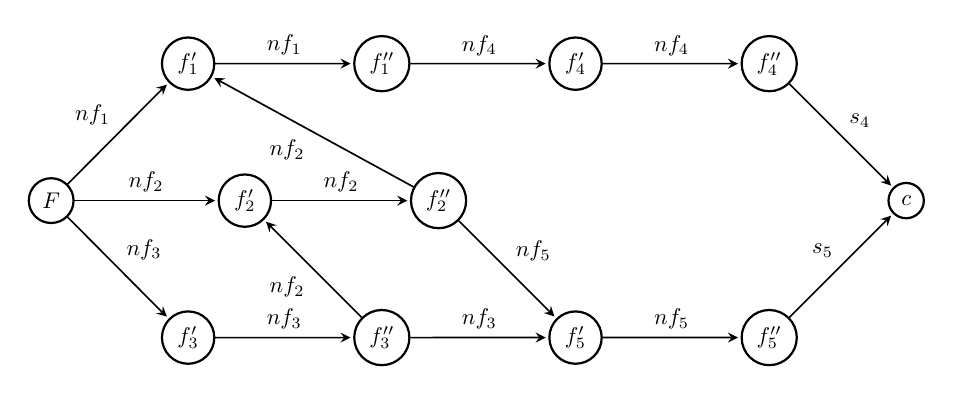
\begin{tikzpicture}[
            > = stealth, % arrow head style
            shorten > = 1pt, % don't touch arrow head to node
            auto,
            node distance = 3cm, % distance between nodes
            semithick,% line style
        	scale=0.85, every node/.style={scale=0.82}
        ]

        \tikzstyle{every state}=[
            draw = black,
            thick,
            fill = white,
            minimum size = 4mm
        ]
        
        % Nodi di F
        \node[state] (F) {$F$};
        \node[state] (f1') 	[above right of=F] 	{$f_1'$};
        \node[state] (f2') 	[right of=F] 		{$f_2'$};   
        \node[state] (f3')  	[below right of=F] 	{$f_3'$};
        \path[->] 	(F) edge node {$nf_1$} (f1');
        \path[->] 	(F) edge node {$nf_2$} (f2');
        \path[->] 	(F) edge node {$nf_3$} (f3');
        
        \node[state] (f3'')	[right of=f3']		{$f_3''$};
        \path[->] 	(f3') edge node {$nf_3$} (f3'');
        \path[->]	(f3'') edge node {$nf_2$} (f2'); % era infinito
        
        \node[state] (f1'') [right of=f1']		{$f_1''$};
        \path[->]	(f1')	edge node {$nf_1$}	(f1'');
      
        
        \node[state]	(f4')	[right of=f1'']	{$f_4'$};
        \path[->]	(f1'')	edge node {$nf_4$}	 (f4');	% era infinito
        
        \node[state]	(f5')	[right of=f3'']	{$f_5'$};
        \path[->]	(f3'')	edge node {$nf_3$}	 (f5');	% era infinito
        
        \node[state]	(f5'')	[right of = f5']	{$f_5''$};
        \path[->]	(f5')	edge node {$nf_5$}	 (f5''); 
        
        \node[state]	(f2'')	[right of=f2']	{$f_2''$};
        \path[->]	(f2') edge node {$nf_2$}	(f2'');
         \path[->]	(f2'')	edge node {$nf_2$}	(f1');	% era infinito
      	\path[->]	(f2'')	edge node {$nf_5$}	 (f5');	% era infinito
	
	\node[state]	(f4'')	[right of = f4']	{$f_4''$};
	\path[->]	(f4')	edge node {$nf_4$}	(f4'');
	
	\node[state]	(c)	[above right of=f5'']	{$c$};
	\path[->]	(f4'')	edge node {$s_4$}	(c);
	\path[->]	(f5'')	edge node {$s_5$}	(c);
	 
\end{tikzpicture}
\captionof{figure}{\textbf{Example with $|F|=5$}}
\end{figure}

\noindent\dotfill
\\In the second part of the exercise, are added some restritions that limit the weekly quantity of chocolate sold there in $c_B$.\\ To deal with this problem, some changes will be made to the main model adding a node to each building.\\
For each building, a node with only one outgoing edge of capacity $c_B$ is added to the sink and all other friends who sell associated with this building have an edge towards the node associated with that building of capacity $s_f$. To add the buildings to the problem formulation just add this definition to the previous graph and to find the number of chocolates to sell, you can use the \textit{Ford Fulkerson} algorithm, which is a \textit{max flow} algorithm that allows to find the maximum flow that crosses a graph from one point to another of this.\\

For the second part of this exercise points 1-4 must be repeated and:
\begin{enumerate}
	\setlength{\itemsep}{1pt}
	\skipitems{4}
	\item For each building in $B$, create a regular node $b_i$ and an edge from it to the sink "Clients" with capacity $c_{b_i}$.
	\item For each friend $f_i \in F$ create an edge from $f_{iB}$ to the node $b_x$, that represent his associated building, with capacity $s_i$.
\end{enumerate}

%1) Definizione rete:
%	- una source (federico)
%	- un sinka
%	- forall amico di federico 2 nodi perché tra i due nodi dell'amico ci sarà un'arco con capacità il nuumero di cioccolatini nf che può gestire un amico.
%	- tutti gli archi devono andare dal secondo nodo di un amico al primo dell'altro (quando ci sono 2 amici che si incontrano) (simmetrica)
%	- la capacità è sempre nf in base all'amico in cui vai nf_1 amico 1, ...
%
%Esempio punto a) |F| = 5
%
%
%
%2) Building:
%	- viene aggiunto un nodo ad ogni building
%	- per ogni building viene aggiunto un nodo con un solo arco uscente di capacità c_b verso il sink e tutti gli altri amici che vendono associati a qual building hanno un arco verso il nodo associato a quel building di capacità s_f.
%	per aggiungere i building alla formulazione del problema basta aggiungere tale def al grafo precedente
%
%Per trovare il numero di cioccolatini da vendere, si potrà usare l'algoritmo ford fulkerson, che è un algoritmo di max_flow

% \begin{minipage}{.4\linewidth}
% \resizebox{\columnwidth}{!}{\begin{tikzpicture}[
%            > = stealth, % arrow head style
%            shorten > = 1pt, % don't touch arrow head to node
%            auto,
%            node distance = 3cm, % distance between nodes
%            semithick% line style
%        ]
%
%        \tikzstyle{every state}=[
%            draw = black,
%            thick,
%            fill = white,
%            minimum size = 4mm
%        ]
%
%        \node[state] (F) {$F$};
%        \node[state] (f1) [above right of=F] {$f_1$};
%        \node[state] (f2) [right of=F] {$f_2$};
%        \node[state] (f3) [below right of=F] {$f_3$};
%        \node[state] (f4) [right of=f1] {$f_4$};
%        \node[state] (f5) [right of=f3] {$f_5$};
%
%        \node[state] (c) [below right of=f4] {$c$};
%
%        \path[->] (F) edge node {$nf_1$} (f1);
%        \path[->] (F) edge node {$nf_2$} (f2);
%        \path[->] (F) edge node {$nf_3$} (f3);
%        \path[->] (f2) edge (f1);
%        \path[->] (f3) edge (f2);
%        \path[->] (f1) edge node {$nf_4$} (f4);
%        \path[->] (f4) edge (c);
%        \path[->] (f3) edge  node {$nf_5$}(f5);
%        \path[->] (f2) edge (f5);
%        \path[->] (f5) edge (c);
%        
%\end{tikzpicture}  
%}
%\end{minipage}
%\begin{minipage}{0.55\linewidth}
%    $Sink$ = $C$ = Customers
%    
%    $f \in F$ = Friends
%    
%    $|F|$ = 5\\
%    
%    $nf_i, \forall f_i \in F$ = Capacity of friend $f_i$\\
%    $sf_i$ = Amount that $f_i$ is able to sell\\
%    $sf \leq nf, nf - ns$ = Amount to be passed
%\end{minipage}
%
%\begin{itemize}[itemsep=.4pt]
%	\item If \textit{C} ask: 0, $f$ produces 0 $\rightarrow v(flow)=0$ 
%	\item If \textit{C} ask: $x < \displaystyle \sum_{i = 1}^3 nf, \ F$ produces $x \rightarrow v(flow) = x$\\
%	\item If \textit{C} ask: $x \geq \displaystyle \sum_{i = 1}^3 nf,\  F$ produces $\displaystyle \sum_{i = 1}^3 nf \rightarrow v(flow) = \displaystyle \sum_{e \ out \ F} c_e$
%	\item $\forall e \in E \rightarrow 0 \leq f(e) \leq c(e) \rightarrow$ capacity condition (i)
%	\item $\forall v \in V-\{F,c\} \rightarrow \displaystyle \sum_{e \ into \ v} f(e)= \displaystyle \sum_{e \ out \ v}f(e) \rightarrow f^{(in)}(v)=f^{(out)}(v) \rightarrow$ Conservation condition (ii)
%	\item $v(flow)=\boxed{f^{out}(F)}= \displaystyle \sum_{e \ out \ F}f(e)$ = Chocolate sold to customers.
%\end{itemize}
%
%Example: \underline{3 Cases}
%\begin{enumerate}
%  \item $C$ ask 100, $\displaystyle \sum_{e \ out \ F}C(e) = 3$\\
%$
%\begin{rcases}
%\begin{aligned}
%  &nf_1 = 1\\
%  &nf_2 = 1 \\
%  &nf_2 = 1 \\
%\end{aligned}
%\end{rcases}
%\ \ \displaystyle \sum_{i=1}^3 nf=3 = \displaystyle \sum_{e \ out \ F} c(e)
%$ \ \ \ \ \ \ \ \ \
%\begin{minipage}{.22\linewidth}
%\resizebox{\columnwidth}{!}{%
%	 \begin{tikzpicture}[
%            > = stealth, % arrow head style
%            shorten > = 1pt, % don't touch arrow head to node
%            auto,
%            node distance = 3cm, % distance between nodes
%            semithick% line style
%        ]
%
%        \tikzstyle{every state}=[
%            draw = black,
%            thick,
%            fill = white,
%            minimum size = 4mm
%        ]
%        \node[state] (F) {$F$};
%        \node[state] (f1) [above right of=F] {$f_1$};
%        \node[state] (f2) [right of=F] {$f_2$};
%        \node[state] (f3) [below right of=F] {$f_3$};
%        \node[state] (f4) [right of=f1] {$f_4$};
%        \node[state] (f5) [right of=f3] {$f_5$};
%
%        \node[state, label=311:{$\frac{3}{100}$}] (c) [below right of=f4] {$c$};
%
%        \path[->] (F) edge node {$1/1$} (f1);
%        \path[->] (F) edge node {$1/1$} (f2);
%        \path[->] (F) edge node {$1/1$} (f3);
%        \path[->] (f2) edge node {0/1} (f1);
%        \path[->] (f3) edge node {$0/1$} (f2);
%        \path[->] (f1) edge node {$1/1$} (f4);
%        \path[->] (f4) edge node {1/1} (c);
%        \path[->] (f3) edge  node {$1/1$}(f5);
%        \path[->] (f2) edge node {1/1} (f5);
%        \path[->] (f5) edge node {1/1} (c);
%         \end{tikzpicture}
%}
%\end{minipage}\\
%
%$f_1, f_2$ and $f_3$ cannot sell, so (i), (ii) must be verified.\\
%$f_4$ and $f_5$ too must verify (i), (ii) and have to sell $sf_4\leq nf_4$ and $sf_5 \leq nf_5$. \\ In this case, to maximize $F'_5$ profit, $sf_4=nf_4$ and $sf_5=nf_5$.
%  \item $C$ ask 0 $\rightarrow v(flow)=0$
%  \item $C$ ask 50, $\displaystyle \sum_{e \ out \ F}c(e) =80$\\
%
%\begin{minipage}{.3\linewidth}	
%$
%\begin{aligned}
%\begin{cases}
%	nf_1=35, \ f^{in}(f_1)=10=f^{out}(f_1)\\
%	nf_2=75, \ f^{in}(f_2)=30=f^{out}(f_2)\\
%	nf_3=25, \ f^{in}(f_3)=15=f^{out}(f_3)\\
%	nf_4=10, \ f^{in}(f_4)=10=f^{out}(f_4)\\
%	nf_5=70, \ f^{in}(f_5)=40=f^{out}(f_5)
%\end{cases}
%\end{aligned}
%$
%\end{minipage}\ \ \  \ \ \ \ \ \ \ \
%\begin{minipage}{.3\linewidth}
%\resizebox{\columnwidth}{!}{%
%	 \begin{tikzpicture}[
%            > = stealth, % arrow head style
%            shorten > = 1pt, % don't touch arrow head to node
%            auto,
%            node distance = 3cm, % distance between nodes
%            semithick% line style
%        ]
%
%        \tikzstyle{every state}=[
%            draw = black,
%            thick,
%            fill = white,
%            minimum size = 4mm
%        ]
%        \node[state] (F) {$F$};
%        \node[state] (f1) [above right of=F] {$f_1$};
%        \node[state] (f2) [right of=F] {$f_2$};
%        \node[state] (f3) [below right of=F] {$f_3$};
%        \node[state] (f4) [right of=f1] {$f_4$};
%        \node[state] (f5) [right of=f3] {$f_5$};
%
%        \node[state] (c) [below right of=f4] {$c$};
%
%        \path[->] (F) edge node {$5/5$} (f1);
%        \path[->] (F) edge node {$30/50$} (f2);
%        \path[->] (F) edge node {$15/25$} (f3);
%        \path[->] (f2) edge node {5/30} (f1);
%        \path[->] (f3) edge node {$0/25$} (f2);
%        \path[->] (f1) edge node {$10/10$} (f4);
%        \path[->] (f4) edge node {10/10} (c);
%        \path[->] (f3) edge  node {$15/25$}(f5);
%        \path[->] (f2) edge node {25/45} (f5);
%        \path[->] (f5) edge node {40/70} (c);
%        \end{tikzpicture}
%}
%\end{minipage}\\
%\end{enumerate}
%
%$f^{out}(f_5)+f^{out}(f_4)=50$ = What $C$ asked, $v(flow)=\displaystyle \sum_{e \ out \ F} f(e)= \boxed{50} \leq \displaystyle \sum_{e \ out \ F}c(e) = \boxed{80}$
%
%\begin{minipage}{.35\linewidth}
% \resizebox{\columnwidth}{!}{\begin{tikzpicture}[
%            > = stealth, % arrow head style
%            shorten > = 1pt, % don't touch arrow head to node
%            auto,
%            node distance = 3cm, % distance between nodes
%            semithick% line style
%        ]
%
%        \tikzstyle{every state}=[
%            draw = black,
%            thick,
%            fill = white,
%            minimum size = 4mm
%        ]
%
%        \node[state] (F) {$F$};
%        \node[state] (f1) [above right of=F] {$f_1$};
%        \node[state] (B1) [above right of=f1] {$B_1$};
%        \node[state] (B2) [right of=f3] {$B_2$};
%        \node[state] (f2) [right of=f1] {$f_2$};
%       	
%       	\node[state] (f4) [right of=F] {$f_4$};
%        \node[state] (f3) [below right of=F] {$f_3$};
%      
%        \node[state] (c) [below right of=f2] {$c$};
%
%        \path[->] (F) edge node {$nf_1$} (f1);
%        \path[->] (F) edge node {$nf_2$} (f2);
%        \path[->] (F) edge node {$nf_4$} (f4);
%        \path[->] (F) edge node {$nf_3$} (f3);
%        \path[->] (f1) edge (B1);
%        \path[->] (f2) edge node {$CB_1$} (B1);
%        \path[->] (f2) edge (f1);
%        \path[->] (f3) edge (f4);
%        \path[->] (f3) edge node {$CB_2$} (B2);
%        	\path[->] (f4) edge (B2);
%        	\path[->] (B2) edge node {$CB_2$} (c);
%        	\path[->] (B1) edge (c);
%        
%\end{tikzpicture}  
%}
%\end{minipage}\ \ \ \ \ \ \
%\begin{minipage}{0.55\linewidth}
%	Same condition as before, but:\\
%	$f_1$ and $f_2$ can only sell MAX $C_{B_{1}}$ in $B_1$\\
%	$f_3$ and $f_4$ can only sell MAX $C_{B_2}$ in $B_2$\\
%	$f^{in}(c) = C_{B_1} + C_{B_2}$\\
%	$v(flow) = \displaystyle \sum_{e \ out \ F}f(e) \leq \displaystyle \sum_{e \ out \ F}c(e)$
%\end{minipage}\\ \\
%
%
%Example:\\
%	 Customers $\in B_1$ ask 1, Customers $\in B_2$ ask 99:\\
%	\begin{minipage}{.10\linewidth}
%		$nf_1 = 20$\\
%		$nf_2 = 40$\\
%		$nf_3 = 10$\\
%		$nf_4 = 60$
%	\end{minipage}\ \ \ \ \ \ \ \ \ \
%	\begin{minipage}{.60\linewidth}
%		, $v(flow) = \displaystyle \sum_{e \ out \ F}f(e) = 61 \leq \displaystyle \sum_{e \ out \ F}c(e) = 116$\\
%		$61 = (F \rightarrow f_3 = 10) + (F \rightarrow f_4 = 50) + (F \rightarrow f_1 = 1)$\\
%		$f_1 \rightarrow B_1 + f_2 \rightarrow B_2 = 1 + 0 = \boxed{\ = C_{B_1}}$\\
%		$f_3 \rightarrow B_2 + f_4 \rightarrow B_4 = 10 +50 = \boxed{60 < C_{B_2}}$\\
%		Sold = 61 < $C_{B_1} + C_{B_2} = 100$
%	\end{minipage}\ \ \
%	\begin{minipage}{.30\linewidth}
%		\resizebox{\columnwidth}{!}{\begin{tikzpicture}[
%            > = stealth, % arrow head style
%            shorten > = 1pt, % don't touch arrow head to node
%            auto,
%            node distance = 3cm, % distance between nodes
%            semithick% line style
%        ]
%
%        \tikzstyle{every state}=[
%            draw = black,
%            thick,
%            fill = white,
%            minimum size = 4mm
%        ]
%
%        \node[state] (F) {$F$};
%        \node[state] (f1) [above right of=F] {$f_1$};
%        \node[state] (B1) [above right of=f1] {$B_1$};
%        \node[state] (B2) [right of=f3] {$B_2$};
%        \node[state] (f2) [right of=f1] {$f_2$};
%       	
%       	\node[state] (f4) [right of=F] {$f_4$};
%        \node[state] (f3) [below right of=F] {$f_3$};
%      
%        \node[state] (c) [below right of=f2] {$c$};
%
%        \path[->] (F) edge node {$1/	10$} (f1);
%        \path[->] (F) edge node {$0/40$} (f2);
%        \path[->] (F) edge node {$50/50$} (f4);
%        \path[->] (F) edge node {$10/10$} (f3);
%        \path[->] (f1) edge node {1/1} (B1);
%        \path[->] (f2) edge node {$0/0$} (B1);
%        \path[->] (f2) edge node{0/10}(f1);
%        \path[->] (f3) edge node{10/10} (f4);
%        \path[->] (f3) edge node {0/0} (B2);
%        \path[->] (f4) edge node {60/60} (B2);
%        \path[->] (B2) edge node {60/60} (c);
%        \path[->] (B1) edge node {1/1}(c);
%        
%\end{tikzpicture}  
%}
%\end{minipage}
%\begin{equation}
%	\begin{cases}
%		nf_1 + nf_2 = 60, C_{B_1} = 1, \text{So } C_{B_1} \text{ limits the deal of } F\\
%		nf_3 +nf_4 = 70, C_{B_2} = 99, C_{B_2} \text{ does not limit the deal but its request is higher than } nf_3 +nf_4\\ \ \ \ \ \ \ \ \ \ \ \ \ \ \ \ \ \ \ \ \ \ \ \ \ \ \ \ \ \ \ \ \ \ \ \ \text{ (Like point A in wich } C \text{ ask } > \displaystyle \sum_{e \ out \ F}c(e)
%	\end{cases}
%\end{equation}


\end{homeworkProblem}

\begin{homeworkProblem}
The problem of the last exercise cannot be solved with a quick algorthm as it must be traced back to an \textit{NP-Complete} problem.\\
The complexity class of decision problems for which answers can be checked for correctness, given a certificate, by an algorithm whose run time is polynomial in the size of the input (that is, it is NP) and no other NP problem is more than a polynomial factor harder.	\\

The problem has as its objective a $k$ value that cannot be exceeded. There is also a set $J$ composed of $n$ tasks and for each $j \in J$ we know beforehand the time $s_j$, the time in which the task $j$, the deadline $d_j$, the time in which it must be terminated must start, and the value $l_j \in N$ which represents the length of the interval to execute the task.Tasks, once started, cannot be paused and deadline $d_j$ is always after the beginning $s_j$.\\
Our problem, through association with the Subset sum Problem, can be associated with the NP-hard type, of which we know that each instance must be solvable.\\
To solve our problem using the known algorithm it is necessary to set some variables. Supposing the valence of the summation $\displaystyle \sum_ {j = 1} ^ {n} l_ {j} = S$ and having a set of integers $I = \{i_1, i_2, ..., i_n\} $ and a value $k$ which represents task, where:

\begin{itemize}[itemsep=1pt, topsep=1pt]
	\item each key $i$ will have $s_{ij}$ (with $j \in N$) which represents the start time set to 0.
	\item each key $i$ will have $d_{ij}$ (with $j \in N$) which in this case represents the deadline set to $S+1$.
	\item Each task $i$ will have $l_{ij}$ (with $j \in N$) which represents the duration initialized to $l_j$.\\
\end{itemize}

Then the Subset sum problem will be able to find a subset of elements from $I$ that will reach $k$.\\
Now we define the $N+1$th task which has a start time equal to $S$, a deadline in $S+1$ and a duration of 1.\\
Having bound the $N+1$th task in the interval $[S, S+1]$ any previous grouping of the subset of tasks that satisfies the sum to $k$, which will also lead to the completion of the $N+1$-th task , will imply the resolution of the objectives by induction in the pre-established time.\\
If each task, which will vary in the subset of 1 to $n$, will be executed within $W$ this will mean that the machine will have no rest time and that the corresponding numbers $l_{i_k}$ in the example of the Subset Sum will reach exactly $W$. Deduces that all tasks were performed before the deadline.\\
To support the previous demonstration, the NP problem definition helps us. In fact, given a possible solution, to consider such a problem it is necessary an efficient certificate of correctness that works in polynomial time.\\
For each instance of the problem, a valid certificate could be the expiration of each task.\\
Having said that, being both a NP-Hard problem and a NP-problem, it has been shown that it is a NP-complete.
\end{homeworkProblem}

\pagebreak

\end{document}
